\documentclass{article}

\usepackage[preprint]{neurips_2024}
\usepackage[utf8]{inputenc}
\usepackage[T1]{fontenc}
\usepackage{hyperref}
\usepackage{url}
\usepackage{booktabs}
\usepackage{graphicx}
\usepackage{amsmath}
\usepackage{amsfonts}
\usepackage{xcolor}
\usepackage{enumitem}
\usepackage{multirow}
\usepackage{tabularx}
\usepackage{array}
\usepackage{placeins}
\usepackage{tikz}
\usetikzlibrary{arrows.meta,positioning,shapes.geometric}
\hypersetup{hidelinks}

\graphicspath{{figures/}}

\makeatletter
\renewcommand{\@notice}{}
\makeatother

\newcommand{\method}[1]{\texttt{\detokenize{#1}}}
\newcommand{\dataset}[1]{\textsc{#1}}
\newcommand{\hyre}{HyRE}
\newcommand{\snaphyre}{Snap-\hyre{}}
\newcolumntype{Y}{>{\raggedright\arraybackslash}X}
\newcolumntype{P}[1]{>{\raggedright\arraybackslash}p{#1}}

\title{\snaphyre{} for Legal RAG: A Source-Gated Results Packet}

\author{%
  Hamza Iqbal \\
  Washington University in St.\ Louis \\
  \texttt{hiqbal@wustl.edu}
  \And
  Hanson Li \\
  Washington University in St.\ Louis \\
  \texttt{hanson.l@wustl.edu}
  \And
  Josh Li \\
  Washington University in St.\ Louis \\
  \texttt{josh.l@wustl.edu}
}

\begin{document}

\maketitle

\begin{abstract}
This draft reports the current fixed-method \snaphyre{} evaluation package for
legal retrieval-augmented generation. \snaphyre{} is a two-call generated-query
method: first produce a tentative legal issue frame and hypothetical reasoning
passage, retrieve with that passage, then answer from the original question and
retrieved corpus evidence. The current signed package is incomplete
(51/84 expected answer cells), so missing rows are left as \textsc{tbd}. In
the signed full-corpus cells, \snaphyre{} improves BarExamQA answer accuracy
over raw RAG for Gemma 4 26B (78.0\% to 82.0\%, $p=0.000699$) and Llama
3.3 70B (74.6\% to 79.8\%, $p=2.70{\times}10^{-5}$). On SCALR and CaseHOLD,
generated retrieval often improves exact Hit@5 while final answer accuracy is
flat or lower. HousingQA currently has raw and oracle rows but no signed
generated-method answer rows. The main claim is therefore intentionally narrow:
retrieval exposure and legal answer accuracy must be reported together, and
\snaphyre{} is currently positive on BarExamQA, mixed on SCALR/CaseHOLD, and
unfinished on HousingQA.
\end{abstract}

\section{Draft Status}

This is a sparse, source-gated paper draft. It treats the current generated
package as the paper's unit of evidence and leaves missing cells visible. The
active framing is a fixed-method \snaphyre{} evaluation, not a dataset-specific
route-selection story. Result claims should continue to be checked against
\method{docs/signoff_log.md}, \method{docs/compiled_results.md},
\method{logs/experiments.jsonl}, and the generated package before submission.

\begin{table}[!htbp]
\centering
\caption{Coverage of the expected 84-cell answer ladder. Generated-method cells are HyDE, Snap-HyRE, and rewrite.}
\label{tab:coverage_matrix}
\scriptsize
\setlength{\tabcolsep}{4pt}
\resizebox{\columnwidth}{!}{%
\begin{tabular}{llcl}
\toprule
Dataset & Model & Signed cells & Missing generated cells \\
\midrule
BarExamQA & Ministral 8B & 4/7 & HyDE, Snap-HyRE, Rewrite \\
BarExamQA & Gemma 4 26B & 7/7 & \textsc{none} \\
BarExamQA & Llama 3.3 70B & 7/7 & \textsc{none} \\
\addlinespace
HousingQA & Ministral 8B & 0/7 & HyDE, Snap-HyRE, Rewrite \\
HousingQA & Gemma 4 26B & 0/7 & HyDE, Snap-HyRE, Rewrite \\
HousingQA & Llama 3.3 70B & 4/7 & HyDE, Snap-HyRE, Rewrite \\
\addlinespace
CaseHOLD & Ministral 8B & 0/7 & HyDE, Snap-HyRE, Rewrite \\
CaseHOLD & Gemma 4 26B & 1/7 & HyDE, Snap-HyRE, Rewrite \\
CaseHOLD & Llama 3.3 70B & 7/7 & \textsc{none} \\
\addlinespace
SCALR & Ministral 8B & 7/7 & \textsc{none} \\
SCALR & Gemma 4 26B & 7/7 & \textsc{none} \\
SCALR & Llama 3.3 70B & 7/7 & \textsc{none} \\
\bottomrule
\end{tabular}}
\end{table}


\section{Method}

\subsection{Evaluation Contract}

The method under test is fixed across datasets and models. We evaluate the same
answer setting at $k=5$ on BarExamQA, HousingQA, CaseHOLD, and
LegalBench-SCALR. We compare seven rows: \method{llm_only},
\method{rag_simple}, \method{rag_hyde}, \method{snap_hyre},
\method{rag_rewrite}, \method{golden_passage}, and
\method{golden_plus_neighbors}. The oracle rows are controls for evidence use,
not deployable methods.

\subsection{Fixed Snap-HyRE}

For each question, the first model call writes a tentative legal issue frame
and a hypothetical reasoning passage. The passage is embedded and used as the
retrieval query. The second model call receives the original question and the
retrieved corpus passages, then emits the final answer. The hypothetical
passage is not treated as evidence in the final call. Older logs may use
\method{rag_snap_hyde_2call}; in this paper that is only a legacy alias for
the same two-call family.

\begin{figure}[!htbp]
\centering
\resizebox{\textwidth}{!}{%
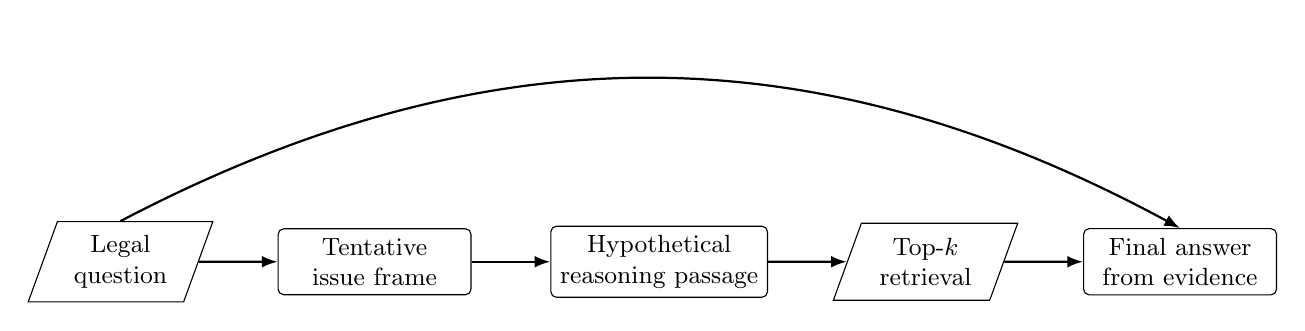
\begin{tikzpicture}[
  node distance=0.9cm and 1.0cm,
  box/.style={draw, rounded corners=2pt, minimum width=2.45cm, minimum height=0.75cm, align=center, font=\small},
  data/.style={draw, trapezium, trapezium left angle=70, trapezium right angle=110, minimum width=2.35cm, minimum height=0.75cm, align=center, font=\small},
  arr/.style={-{Latex[length=2mm]}, thick}
]
\node[data] (q) {Legal\\question};
\node[box, right=of q] (snap) {Tentative\\issue frame};
\node[box, right=of snap] (hyde) {Hypothetical\\reasoning passage};
\node[data, right=of hyde] (ret) {Top-$k$\\retrieval};
\node[box, right=of ret] (final) {Final answer\\from evidence};
\draw[arr] (q) -- (snap);
\draw[arr] (snap) -- (hyde);
\draw[arr] (hyde) -- (ret);
\draw[arr] (ret) -- (final);
\draw[arr, bend left=28] (q.north) to (final.north);
\end{tikzpicture}}
\caption{\snaphyre{} retrieval. Generated text shapes retrieval; final answer
generation is grounded in the original question and retrieved corpus passages.}
\label{fig:method_diagram}
\end{figure}

\subsection{Run Accounting}

Conceptually, \method{rag_hyde}, \method{snap_hyre}, and
\method{rag_rewrite} are two-call methods when run end-to-end. Some answer rows
replay already-built generation and retrieval caches, so answer-package
\method{avg_llm_calls} can show one answer call even for a two-call method.
That field is an answer-run accounting statistic, not the conceptual method
cost.

\subsection{Metrics}

The answer metric is task accuracy. Retrieval exposure is exact-qrel Hit@k and
MRR@k over labeled gold evidence ids or legal holdings. Exact-qrel metrics are
useful but incomplete: they can miss legally equivalent retrieved passages, and
they can overstate usefulness when the gold id appears among strong distractors.
For that reason, the paper reports retrieval metrics, answer accuracy, oracle
evidence controls, and paired McNemar tests together.

This evaluation follows the retrieval-augmented generation and generated-query
line of work \citep{lewis2020rag,gao2023hyde,wang2023query2doc}, applied to
legal benchmarks including LegalBench-SCALR, CaseHOLD, BarExamQA, and
HousingQA \citep{guha2023legalbench,zheng2021casehold,zheng2025legalretrieval}.

\section{Results}

\subsection{Answer Grid}

\begin{table*}[!htbp]
\centering
\caption{Current signed full-corpus answer accuracy at $k=5$ (\%). \textsc{tbd} cells are absent from the current fixed-method package rather than inferred from older runs.}
\label{tab:answer_matrix}
\scriptsize
\setlength{\tabcolsep}{3.8pt}
\resizebox{\textwidth}{!}{%
\begin{tabular}{llrrrrrrr}
\toprule
Dataset / model & $N$ & LLM & Raw RAG & HyDE & Snap-HyRE & Rewrite & Gold & Gold+Nbrs \\
\midrule
BarExamQA / Ministral 8B & 1195 & 56.8 & 56.9 & \textsc{tbd} & \textsc{tbd} & \textsc{tbd} & 64.6 & 63.2 \\
BarExamQA / Gemma 4 26B & 1195 & 80.8 & 78.0 & 80.2 & 82.0 & 80.7 & 78.6 & 80.7 \\
BarExamQA / Llama 3.3 70B & 1195 & 78.7 & 74.6 & 80.2 & 79.8 & 77.2 & 79.2 & 77.8 \\
\addlinespace
HousingQA / Ministral 8B & 6853 & \textsc{tbd} & \textsc{tbd} & \textsc{tbd} & \textsc{tbd} & \textsc{tbd} & \textsc{tbd} & \textsc{tbd} \\
HousingQA / Gemma 4 26B & 6853 & \textsc{tbd} & \textsc{tbd} & \textsc{tbd} & \textsc{tbd} & \textsc{tbd} & \textsc{tbd} & \textsc{tbd} \\
HousingQA / Llama 3.3 70B & 6853 & 44.8 & 47.3 & \textsc{tbd} & \textsc{tbd} & \textsc{tbd} & 67.3 & 66.0 \\
\addlinespace
CaseHOLD / Ministral 8B & 3600 & \textsc{tbd} & \textsc{tbd} & \textsc{tbd} & \textsc{tbd} & \textsc{tbd} & \textsc{tbd} & \textsc{tbd} \\
CaseHOLD / Gemma 4 26B & 3600 & 72.6 & \textsc{tbd} & \textsc{tbd} & \textsc{tbd} & \textsc{tbd} & \textsc{tbd} & \textsc{tbd} \\
CaseHOLD / Llama 3.3 70B & 3600 & 71.8 & 70.8 & 70.3 & 70.5 & 70.6 & 97.5 & 79.4 \\
\addlinespace
SCALR / Ministral 8B & 571 & 67.2 & 68.0 & 71.1 & 69.9 & 69.9 & 93.2 & 77.1 \\
SCALR / Gemma 4 26B & 571 & 73.0 & 73.4 & 72.2 & 73.9 & 73.9 & 97.9 & 81.3 \\
SCALR / Llama 3.3 70B & 571 & 74.4 & 72.9 & 70.4 & 71.3 & 71.6 & 93.5 & 83.0 \\
\bottomrule
\end{tabular}}
\end{table*}


\begin{table}[!htbp]
\centering
\caption{Unbalanced averages across completed clean answer cells. These means summarize the current package only; they are not benchmark-balanced leaderboard scores.}
\label{tab:completed_means}
\scriptsize
\setlength{\tabcolsep}{4pt}
\begin{tabular}{lrrr}
\toprule
Mode & Cells & Mean acc. & Mean $\Delta$ vs raw \\
\midrule
LLM-only & 9 & 68.9 & 0.7 \\
Raw RAG & 8 & 67.7 & 0.0 \\
HyDE & 6 & 74.1 & 1.2 \\
Snap-HyRE & 6 & 74.6 & 1.6 \\
Rewrite & 6 & 74.0 & 1.1 \\
Gold & 8 & 84.0 & 16.3 \\
Gold+Nbrs & 8 & 76.1 & 8.3 \\
\bottomrule
\end{tabular}
\end{table}


The completed-cell means are only an orientation check because the grid is
unbalanced. The safer result object is Table~\ref{tab:answer_matrix}: BarExamQA
has two signed positive \snaphyre{} cells, SCALR has mixed generated-query
answer behavior, CaseHOLD has a signed Llama 70B row with little answer
conversion, and HousingQA generated-method answer rows remain \textsc{tbd}.

\begin{figure}[!htbp]
  \centering
  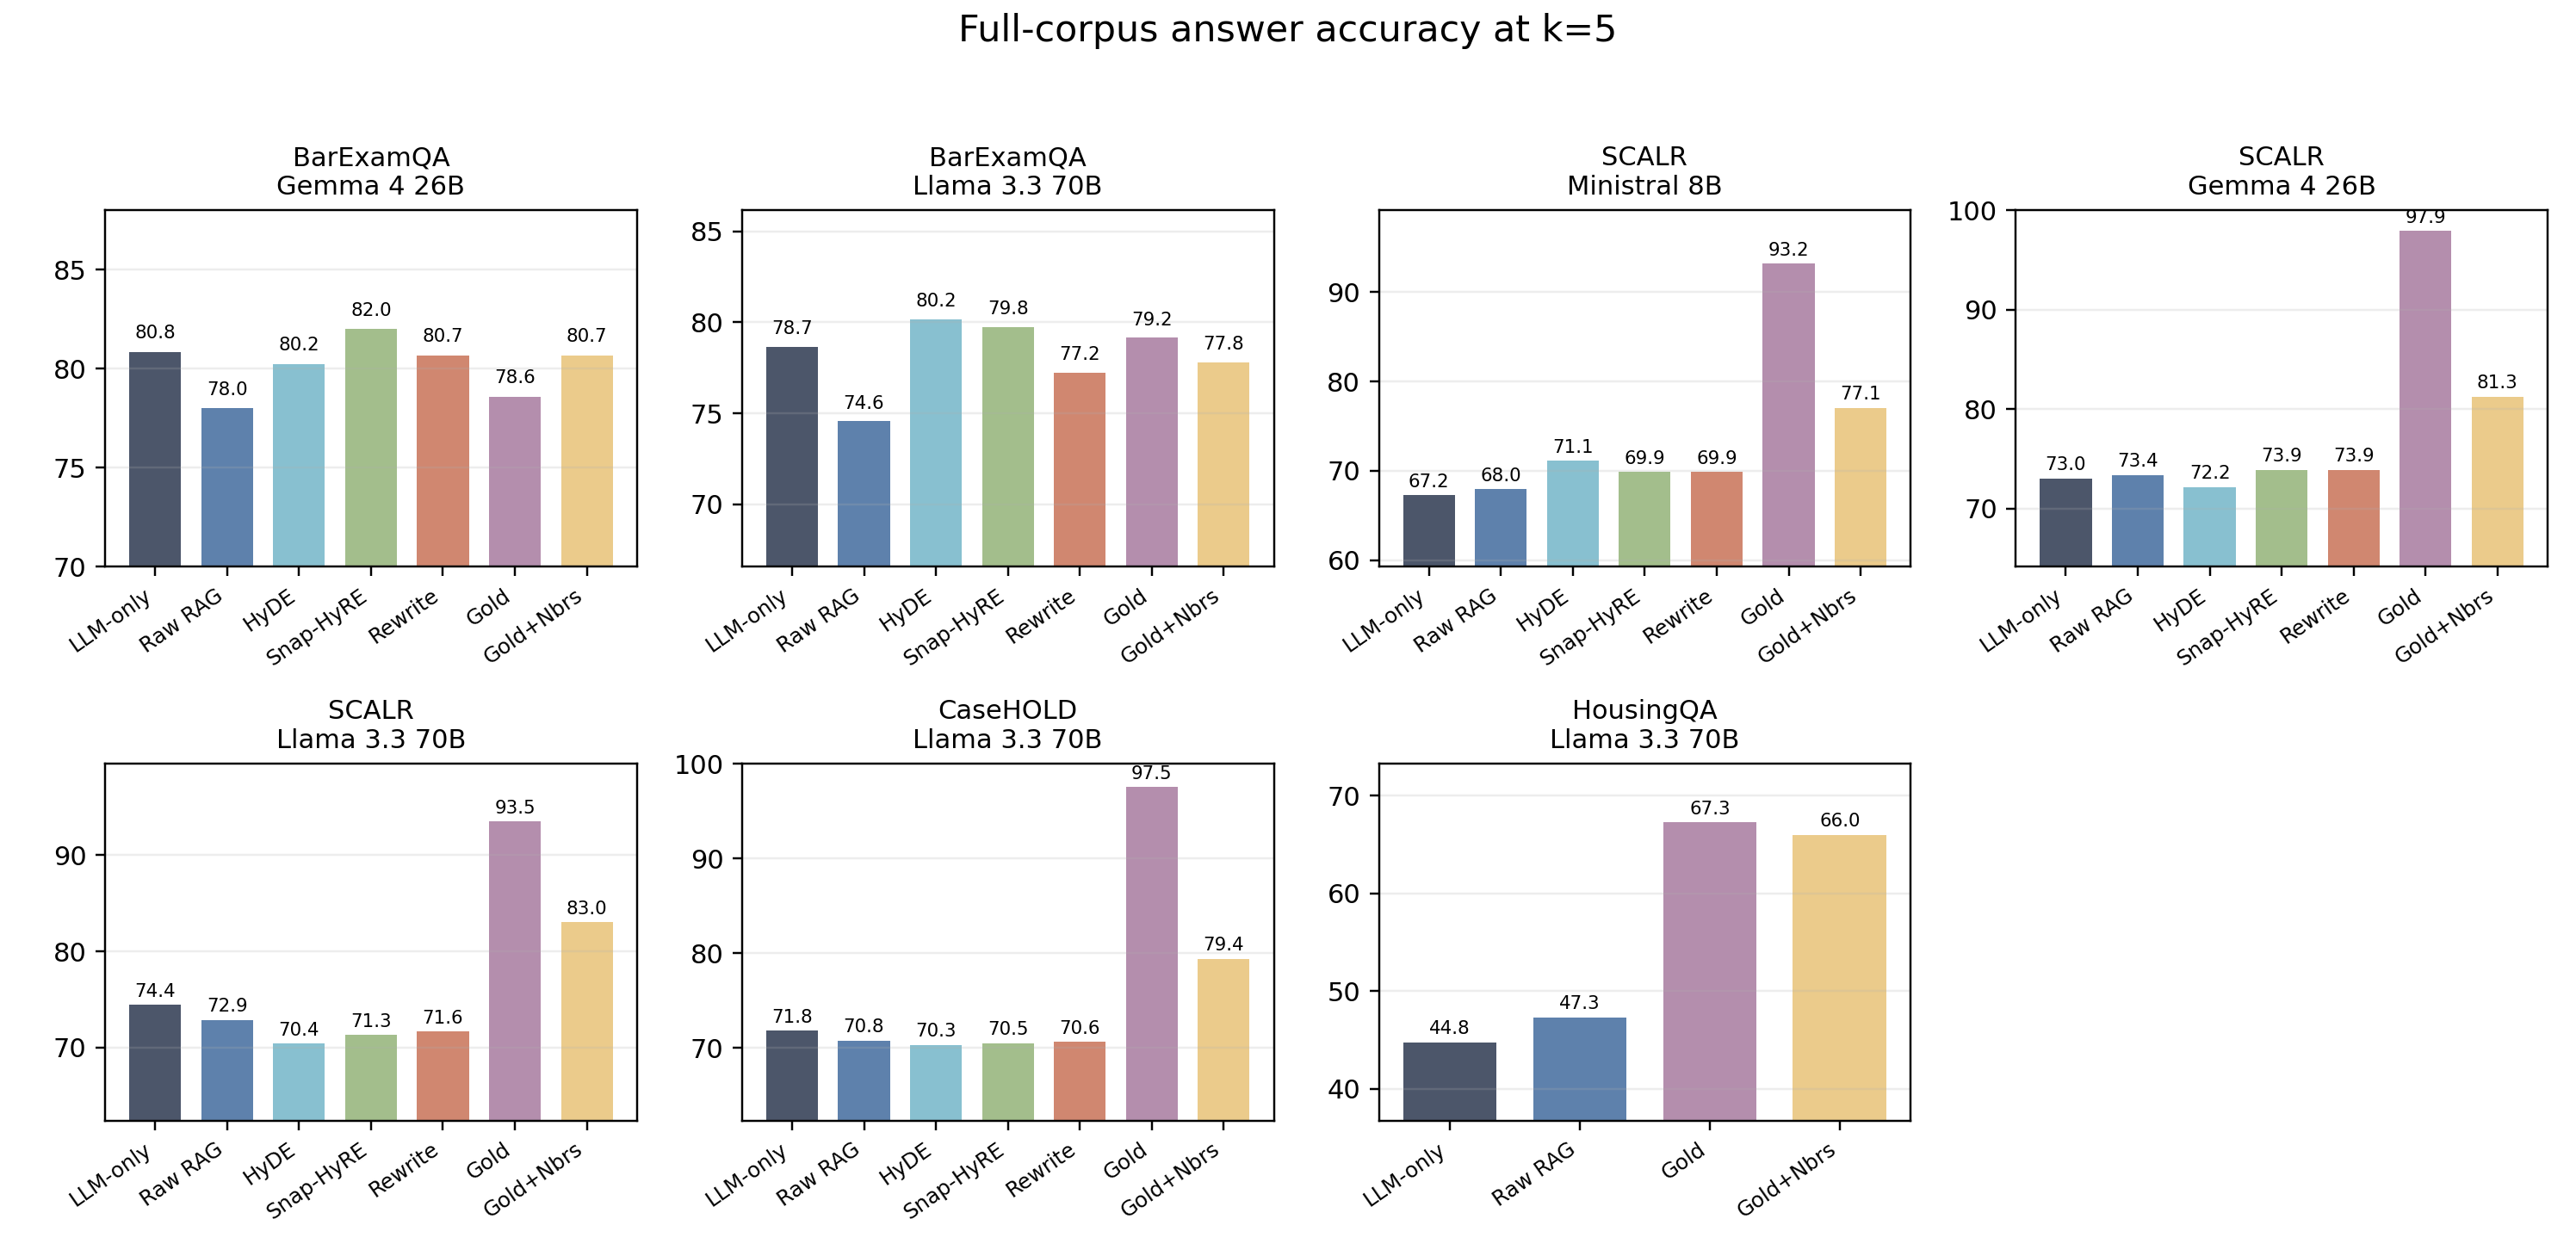
\includegraphics[width=\textwidth]{01_answer_ladder_by_dataset.png}
  \caption{Answer ladders for currently signed cells. This figure is a visual
  companion to Table~\ref{tab:answer_matrix}; missing cells are omitted rather
  than filled from older runs.}
  \label{fig:answer_ladder}
\end{figure}

\FloatBarrier

\subsection{Retrieval and Answer Conversion}

\begin{table*}[!htbp]
\centering
\caption{Retrieval exposure and answer conversion at $k=5$ for RAG-simple, HyDE, Snap-HyRE, and RAG-rewrite rows with signed full answer and retrieval results. Deltas are method answer accuracy minus the RAG-simple answer accuracy in the same dataset/model cell.}
\label{tab:method_conversion}
\scriptsize
\setlength{\tabcolsep}{4pt}
\resizebox{\textwidth}{!}{%
\begin{tabular}{llrrrrrrrr}
\toprule
Dataset & Model & \multicolumn{2}{c}{\method{rag_simple}} & \multicolumn{2}{c}{\method{rag_hyde}} & \multicolumn{2}{c}{\method{snap_hyre}} & \multicolumn{2}{c}{\method{rag_rewrite}} \\
\cmidrule(lr){3-4}\cmidrule(lr){5-6}\cmidrule(lr){7-8}\cmidrule(lr){9-10}
 & & Hit@5 & Acc. & Hit@5 & $\Delta$ Acc. & Hit@5 & $\Delta$ Acc. & Hit@5 & $\Delta$ Acc. \\
\midrule
BarExamQA & Gemma 4 26B & 1.4 & 78.0 & 11.4 & +2.26 & 12.1 & +4.02 & 12.2 & +2.68 \\
BarExamQA & Llama 3.3 70B & 1.4 & 74.6 & 10.5 & +5.61 & 11.1 & +5.19 & 12.2 & +2.68 \\
SCALR & Ministral 8B & 49.6 & 68.0 & 60.3 & +3.15 & 62.0 & +1.93 & 65.0 & +1.93 \\
SCALR & Gemma 4 26B & 49.6 & 73.4 & 70.8 & -1.23 & 72.7 & +0.53 & 67.4 & +0.53 \\
SCALR & Llama 3.3 70B & 49.6 & 72.9 & 61.5 & -2.45 & 55.2 & -1.57 & 57.6 & -1.22 \\
CaseHOLD & Llama 3.3 70B & 17.9 & 70.8 & 51.2 & -0.42 & 45.0 & -0.25 & 45.1 & -0.14 \\
HousingQA & Llama 3.3 70B & \textsc{tbd} & 47.3 & \textsc{tbd} & \textsc{tbd} & \textsc{tbd} & \textsc{tbd} & \textsc{tbd} & \textsc{tbd} \\
\bottomrule
\end{tabular}}
\end{table*}


Table~\ref{tab:method_conversion} is the central failure-analysis table. It
compares \method{rag_simple}, \method{rag_hyde}, \method{snap_hyre}, and
\method{rag_rewrite}; the generated-method deltas are answer-accuracy changes
relative to \method{rag_simple} in the same dataset/model cell. On BarExamQA,
generated retrieval handles improve RAG-simple retrieval exposure and
\snaphyre{} improves answer accuracy. On SCALR and CaseHOLD, higher exact
Hit@5 often fails to become higher final accuracy. This is the main reason the
paper should avoid a simple retrieval-win narrative.

\begin{figure}[!htbp]
  \centering
  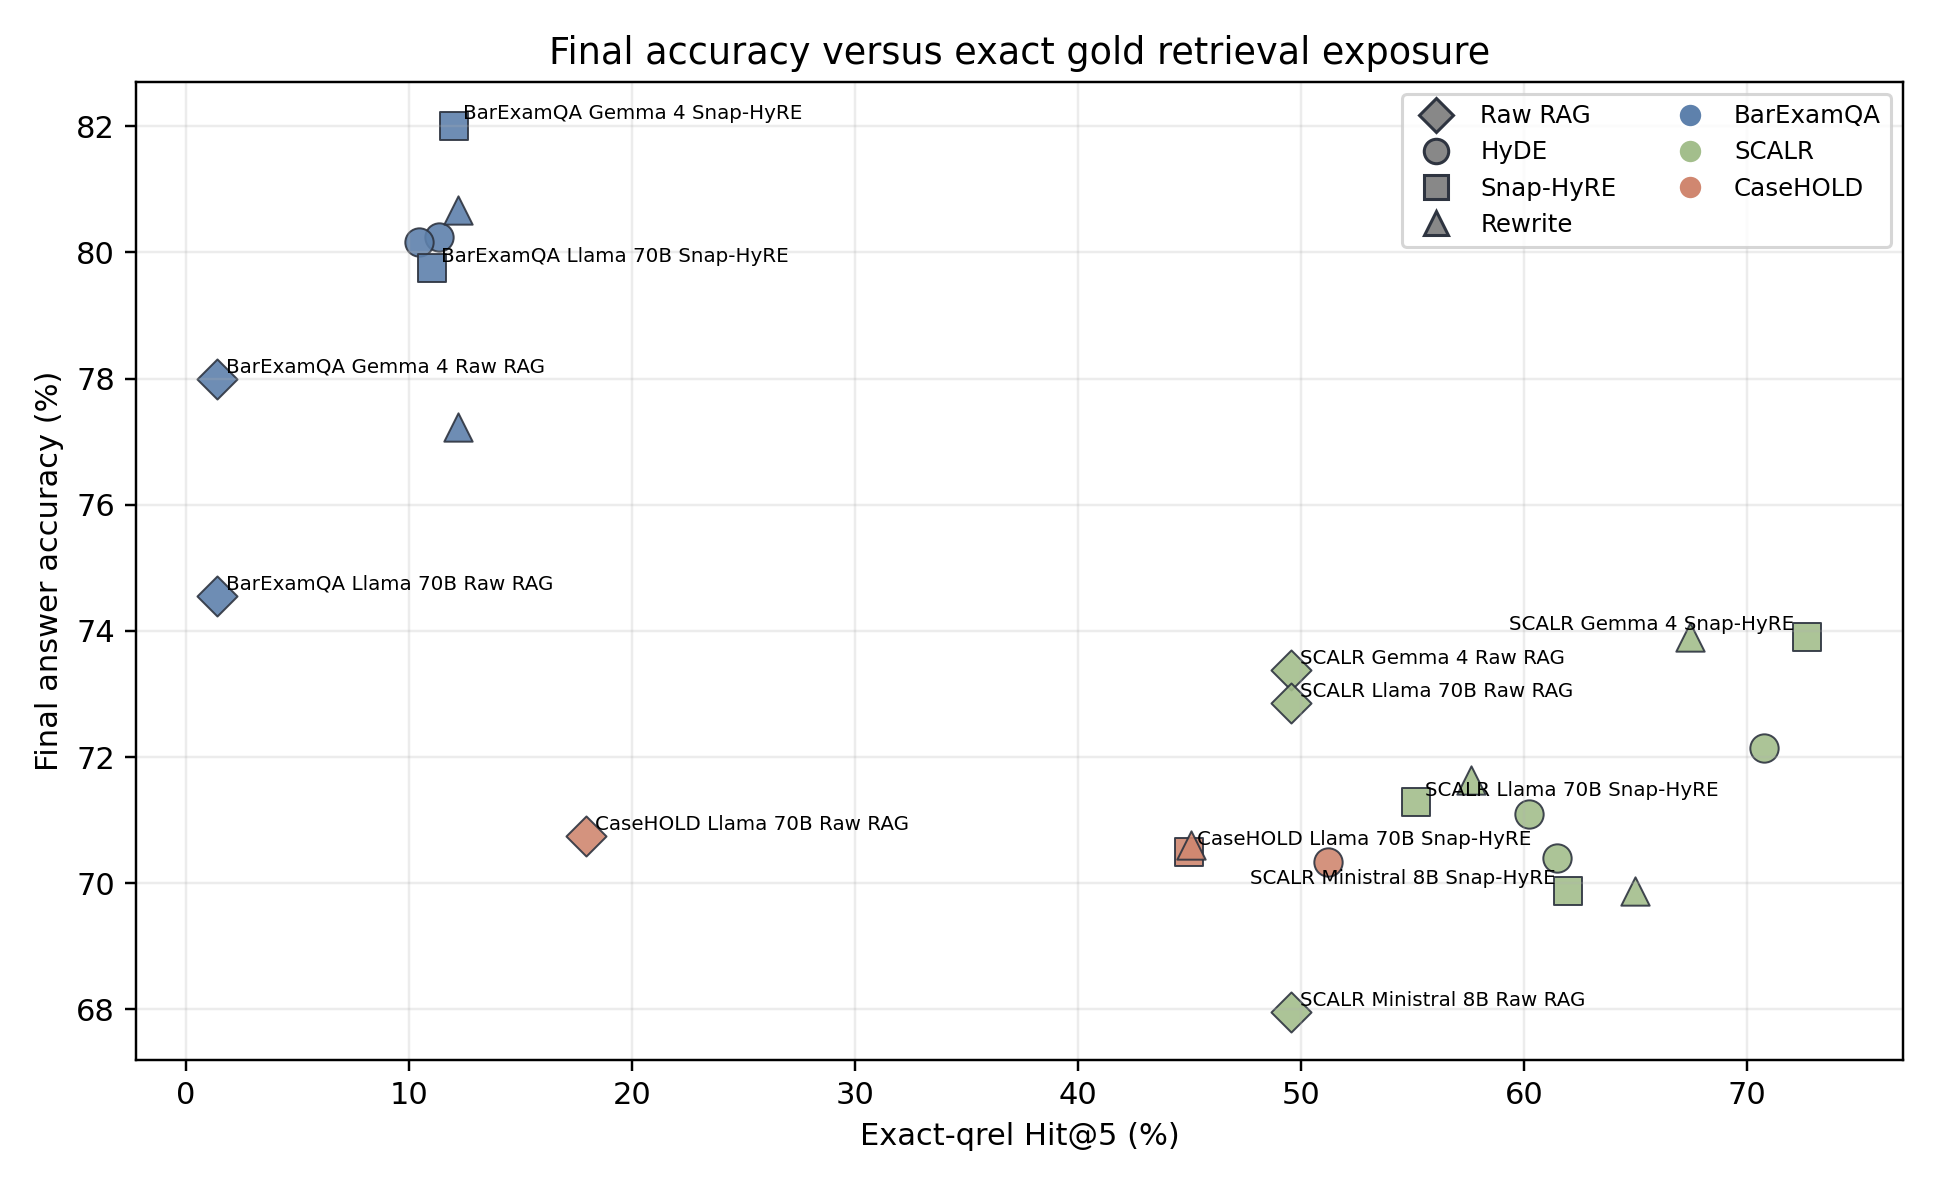
\includegraphics[width=0.88\textwidth]{02_accuracy_vs_hit5.png}
  \caption{Final answer accuracy versus exact-qrel Hit@5 for signed
  generated-query cells and their raw-RAG baselines. The same retrieval lift can
  correspond to positive, flat, or negative answer movement.}
  \label{fig:accuracy_vs_hit5}
\end{figure}

\begin{table*}[!htbp]
\centering
\caption{Paired McNemar comparisons for Snap-HyRE against selected controls. Deltas are percentage points in answer accuracy.}
\label{tab:snap_significance}
\scriptsize
\setlength{\tabcolsep}{4pt}
\resizebox{\textwidth}{!}{%
\begin{tabular}{llrrrrrr}
\toprule
Dataset & Model & $\Delta$ raw & $p$ raw & $\Delta$ LLM & $p$ LLM & $\Delta$ HyDE & $p$ HyDE \\
\midrule
BarExamQA & Gemma 4 26B & +4.02 & 0.000699 & +1.17 & 0.348 & +1.76 & 0.0987 \\
BarExamQA & Llama 70B & +5.19 & 2.70e-05 & +1.09 & 0.388 & -0.42 & 0.754 \\
SCALR & Ministral 8B & +1.93 & 0.260 & +2.63 & 0.110 & -1.23 & 0.457 \\
SCALR & Gemma 4 26B & +0.53 & 0.780 & +0.88 & 0.560 & +1.75 & 0.220 \\
SCALR & Llama 70B & -1.58 & 0.281 & -3.15 & 0.0222 & +0.88 & 0.542 \\
CaseHOLD & Llama 70B & -0.25 & 0.722 & -1.31 & 0.0295 & +0.17 & 0.812 \\
\bottomrule
\end{tabular}}
\end{table*}


\FloatBarrier

\subsection{Oracle Evidence Controls}

Oracle rows separate retrieval failure from evidence-use failure. Gold-only
accuracy is very high on SCALR and CaseHOLD, but gold-plus-neighbors is lower
than gold-only, showing that extra plausible legal text can dilute the signal.
HousingQA also has a large oracle gap: Llama 70B raw RAG is 47.3\%, while
gold-only is 67.3\%.

\begin{figure}[!htbp]
  \centering
  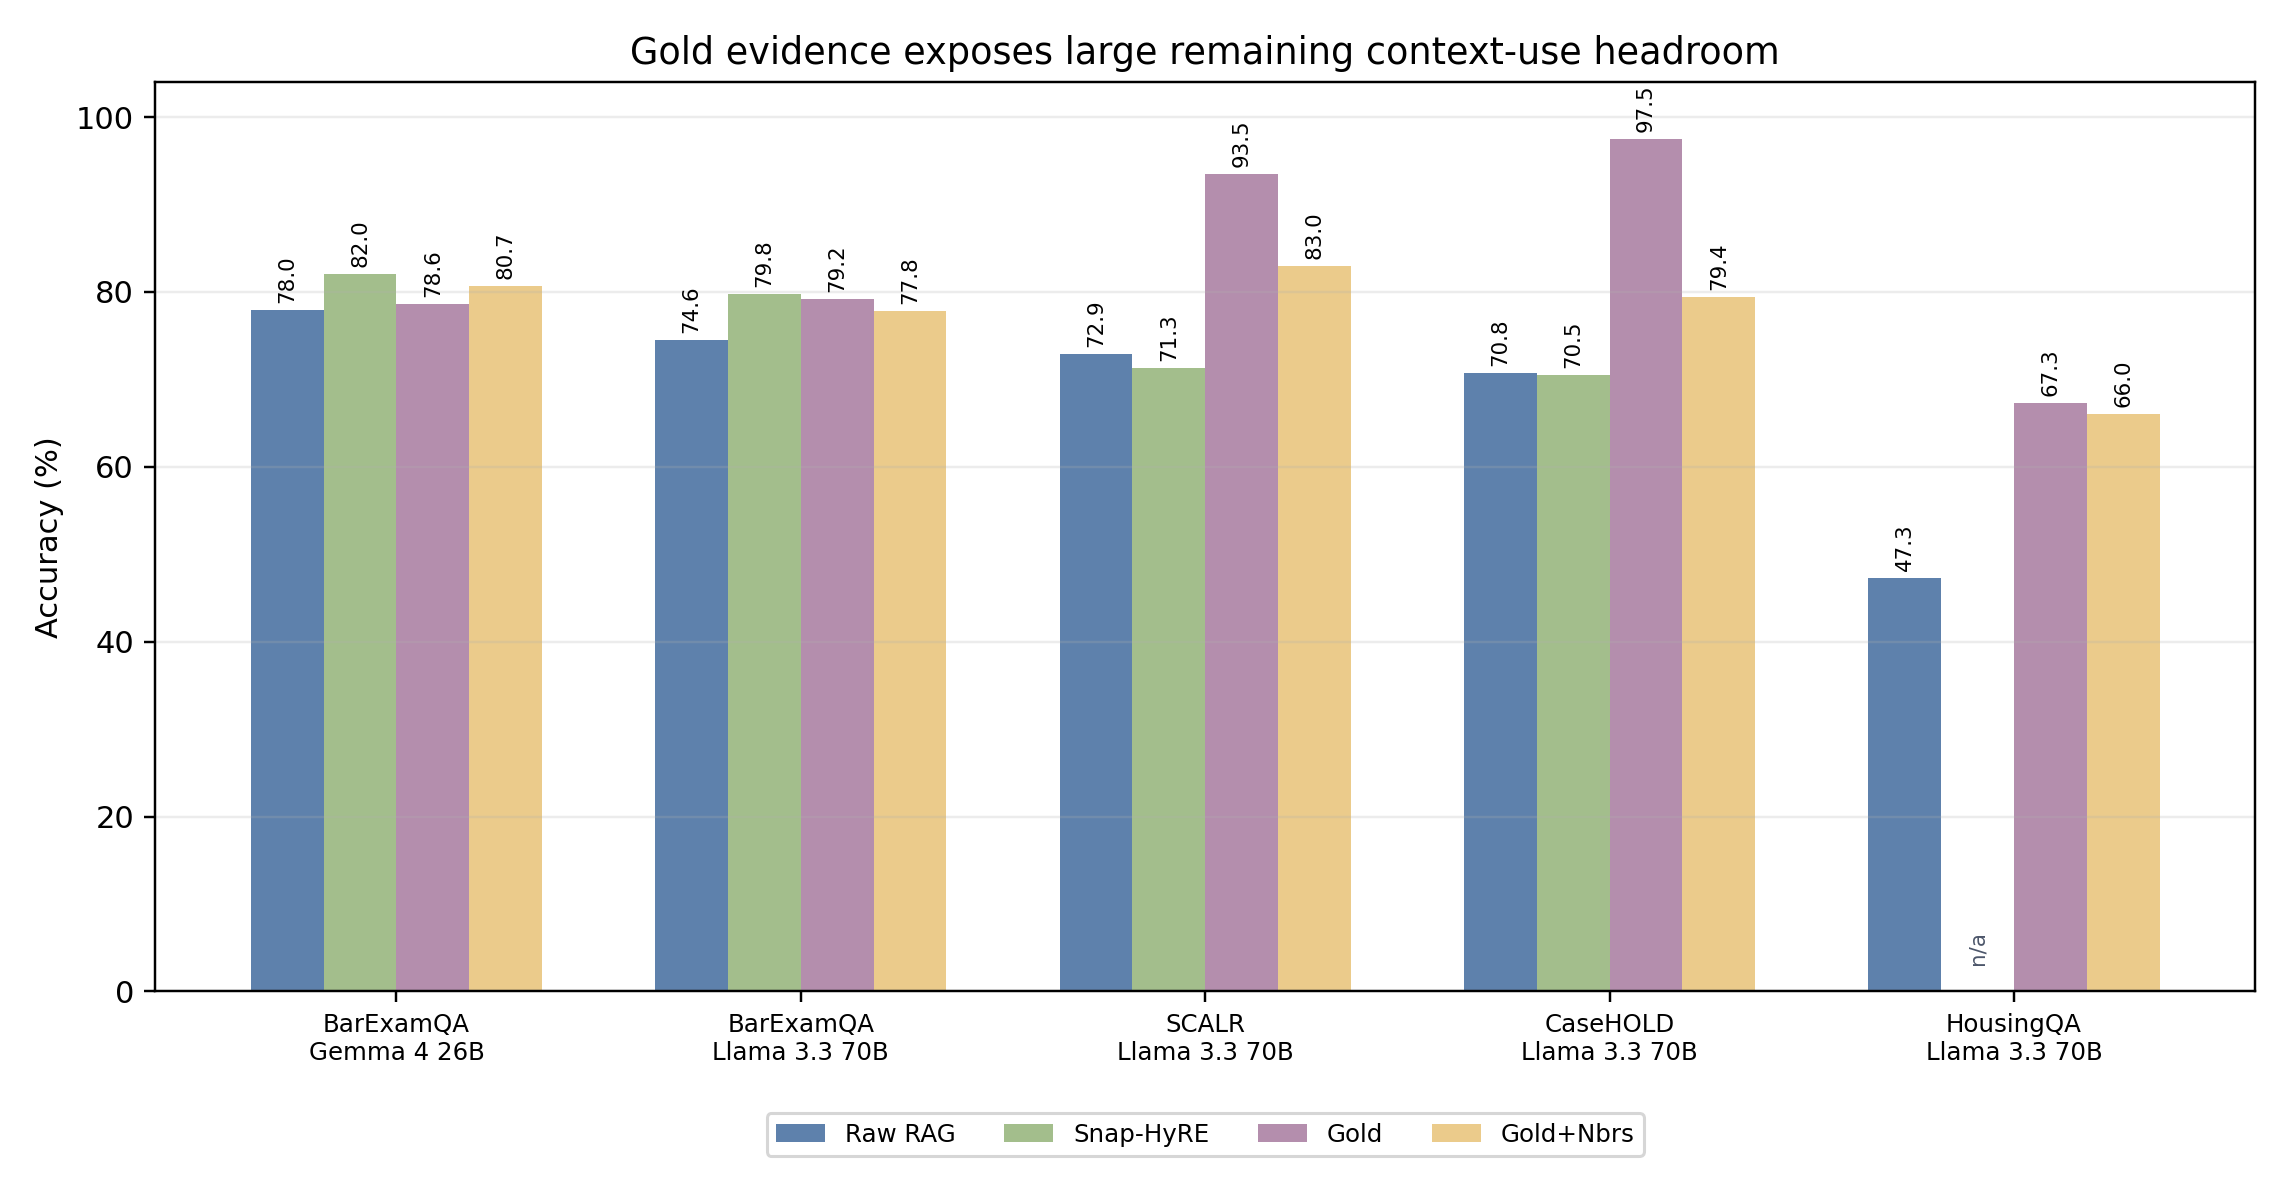
\includegraphics[width=0.90\textwidth]{03_oracle_gap.png}
  \caption{Oracle evidence controls expose remaining context-use headroom.
  Gold-plus-neighbor rows should not be read as an oracle ceiling; they also
  test distractor sensitivity.}
  \label{fig:oracle_gap}
\end{figure}

\FloatBarrier

\subsection{Top-k Analyses}

The main answer grid uses $k=5$. Retrieval curves through $k=10$ are still
reported because they show whether generated-query methods move gold evidence
into the candidate set. The q100 prelaunch probe is not a final top-k
benchmark; it only justifies using $k=5$ as the shared answer setting while
retaining k-curves for analysis.

\begin{table}[!htbp]
\centering
\caption{q100 prelaunch top-$k$ probe. Retrieval exposure rises after $k=5$, but MRR changes little and BarExamQA downstream accuracy did not favor $k=10$.}
\label{tab:q100_topk_probe}
\scriptsize
\setlength{\tabcolsep}{4pt}
\begin{tabular}{rrrr}
\toprule
$k$ & Macro Hit@k & Macro MRR@k & BarExam q100 acc. \\
\midrule
1 & 19.5 & 0.195 & \textsc{n/a} \\
5 & 31.7 & 0.239 & raw 83, HyDE 87 \\
10 & 36.2 & 0.245 & raw 81, HyDE 84 \\
\bottomrule
\end{tabular}
\end{table}


\begin{figure}[!htbp]
  \centering
  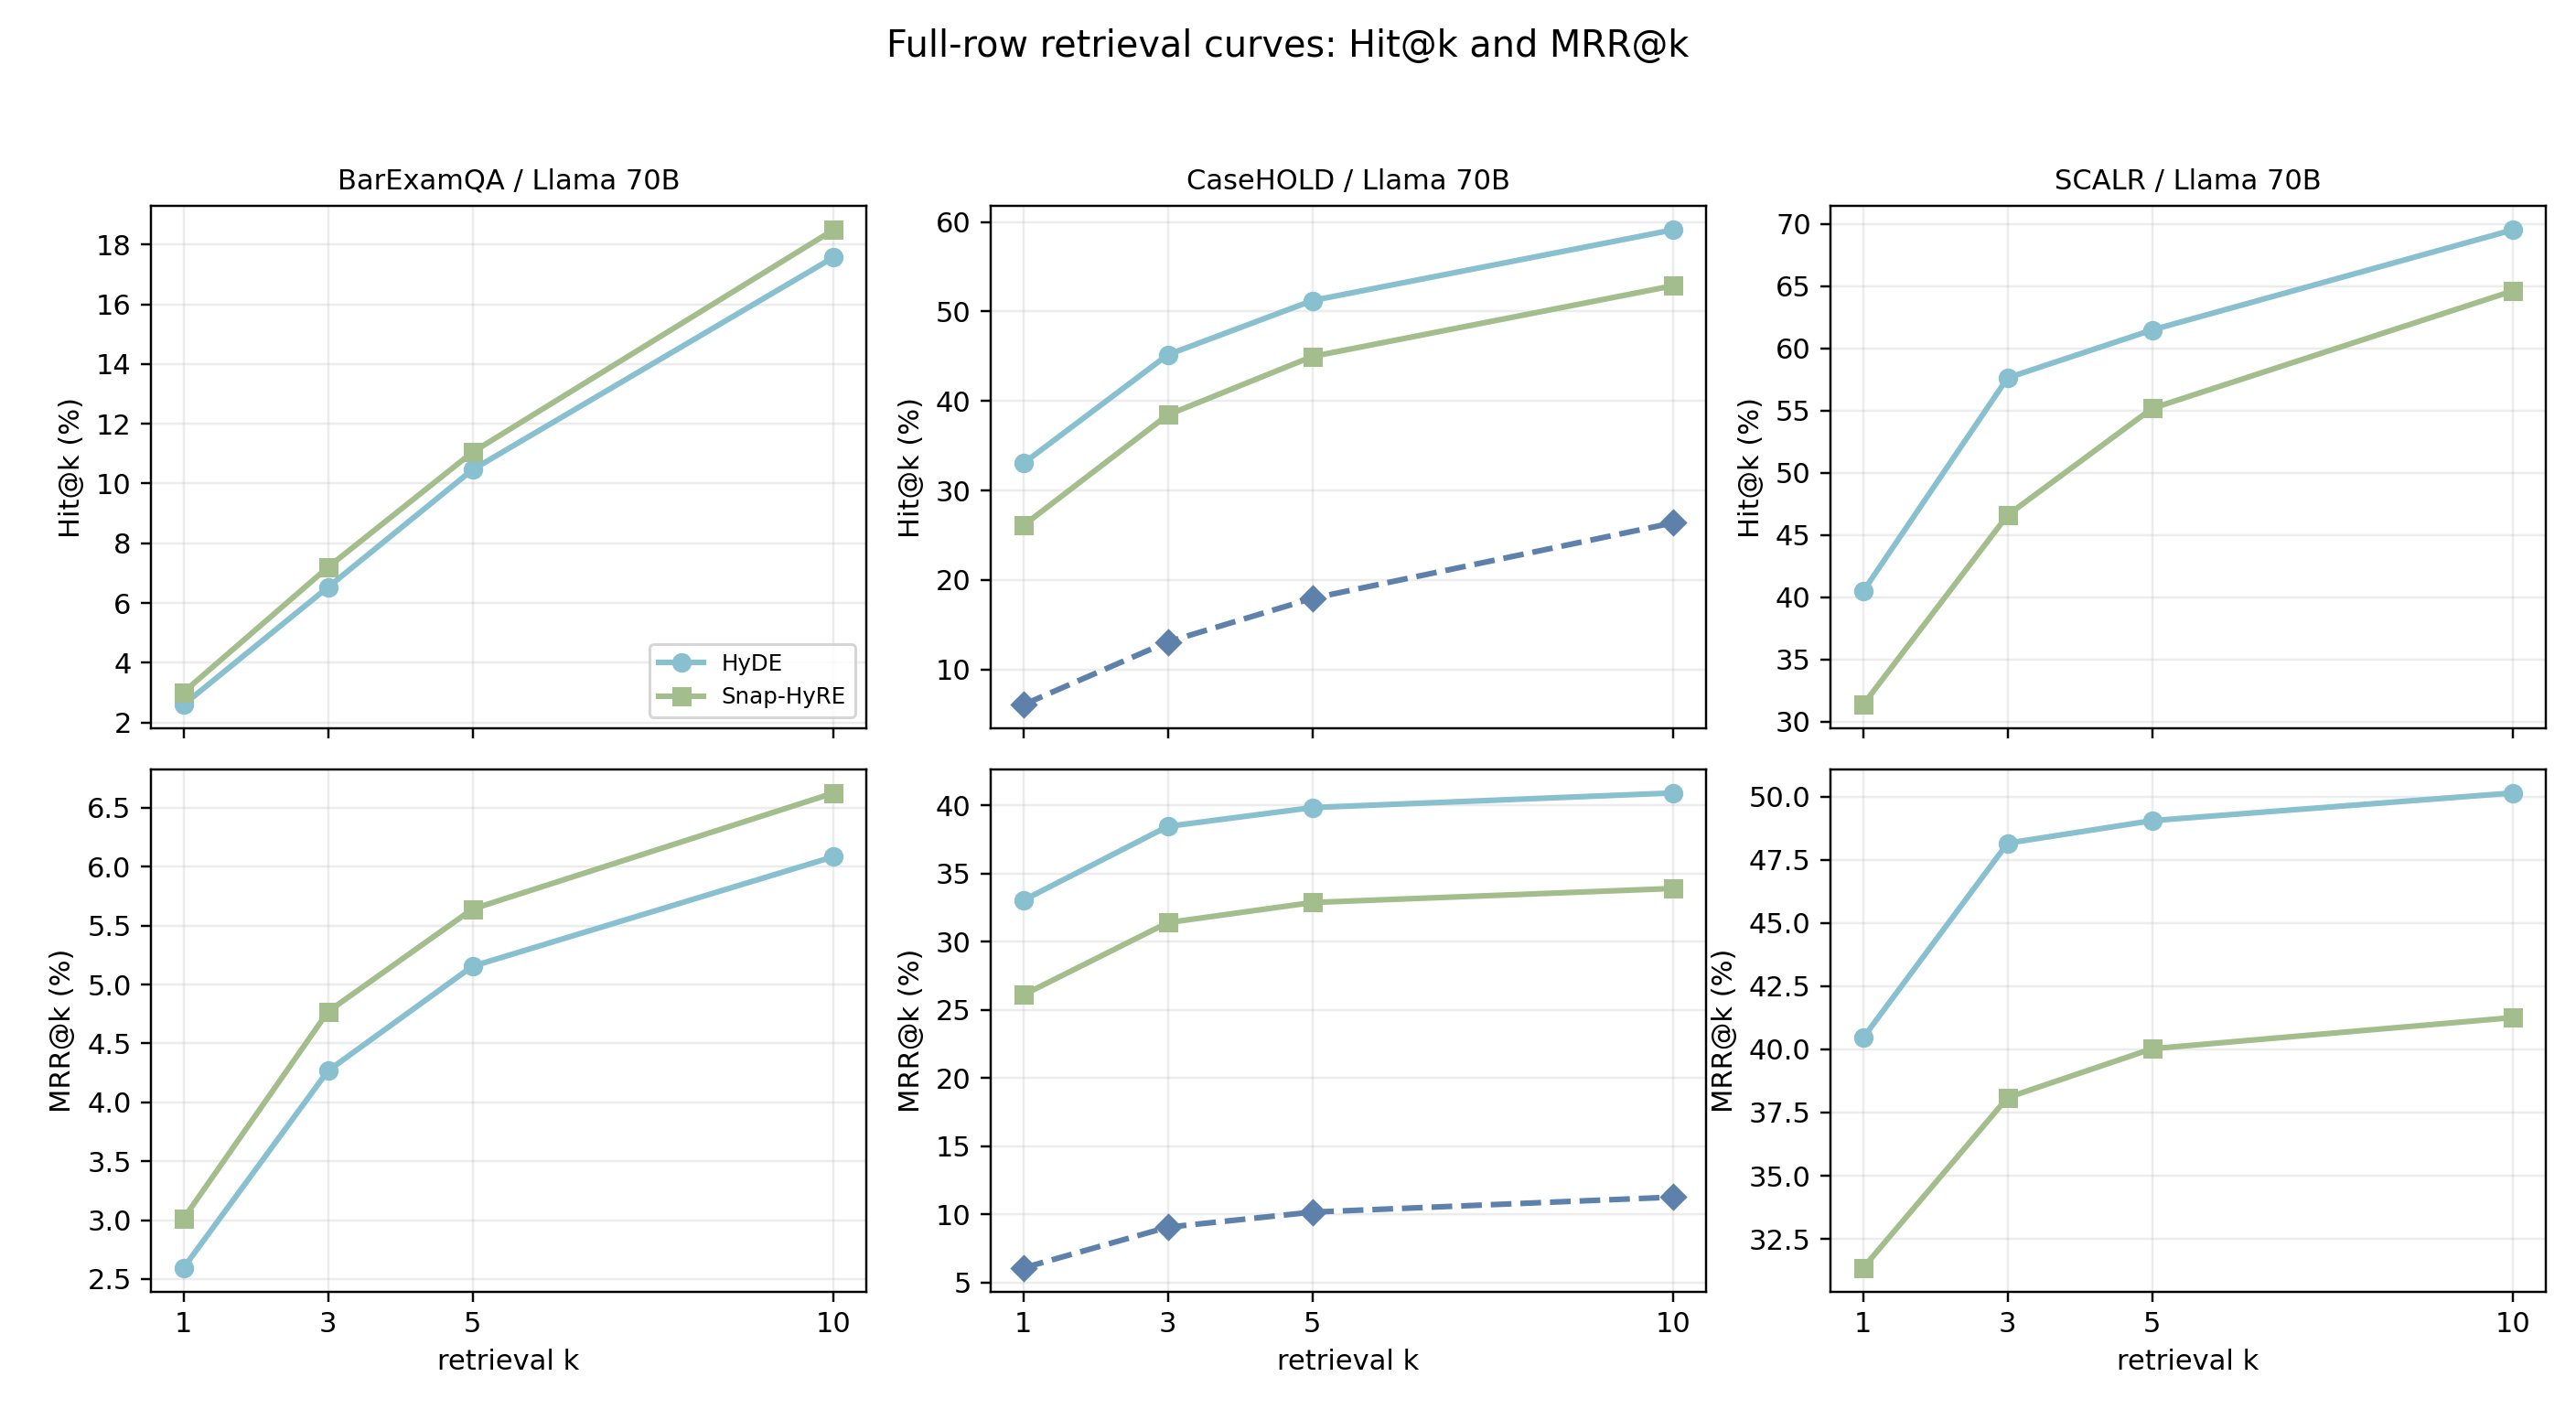
\includegraphics[width=\textwidth]{04_retrieval_hit_mrr_curves_full.png}
  \caption{Full-row retrieval curves for signed caches with at least 500 rows.
  Hit@k and MRR@k are shown separately; raw full curves are available in this
  package for CaseHOLD and are otherwise summarized at k=5 in
  Table~\ref{tab:method_conversion}.}
  \label{fig:retrieval_hit_mrr}
\end{figure}

\begin{figure}[!htbp]
  \centering
  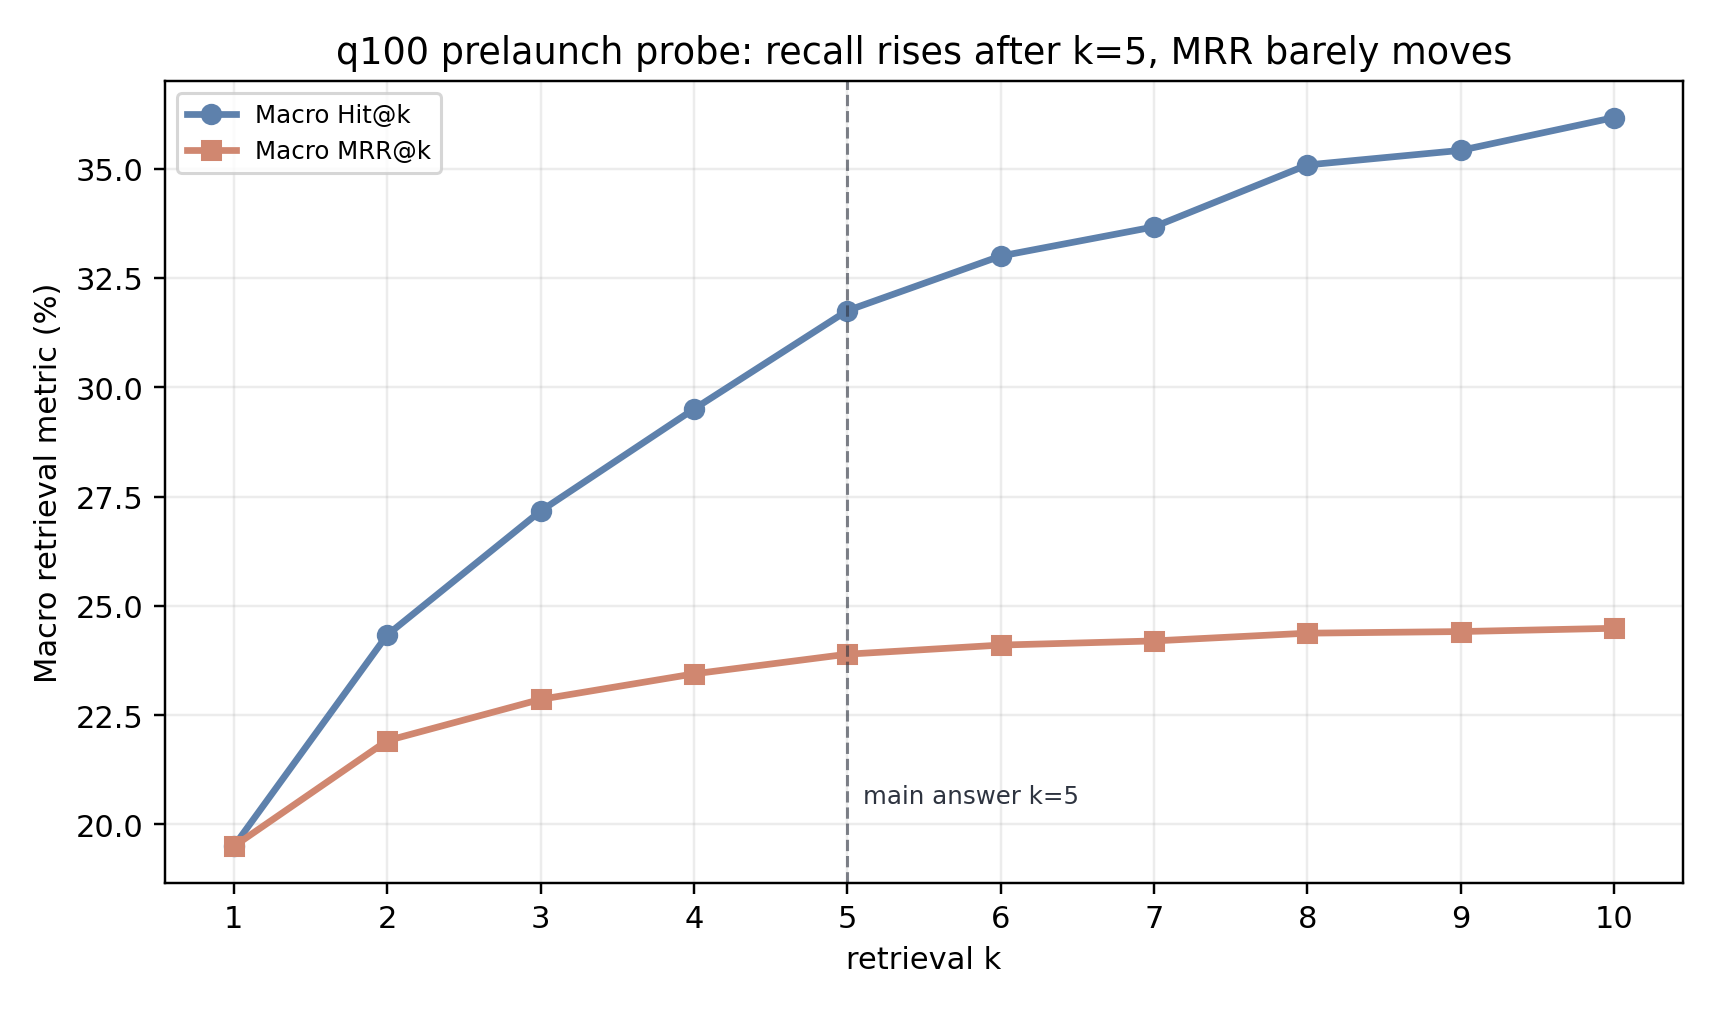
\includegraphics[width=0.78\textwidth]{05_q100_macro_topk_probe.png}
  \caption{q100 prelaunch retrieval probe over supplied Gemma 4 26B caches.
  Macro Hit@k rises after k=5, while MRR changes little; the small downstream
  BarExamQA check did not favor k=10.}
  \label{fig:q100_probe}
\end{figure}

\FloatBarrier

\subsection{Row Caveats}

\begin{table*}[!htbp]
\centering
\caption{Caveats that should travel with exact row claims. Detailed provenance remains in the signoff log.}
\label{tab:caveat_ledger}
\scriptsize
\setlength{\tabcolsep}{4pt}
\begin{tabularx}{\textwidth}{lllY}
\toprule
Dataset & Model & Row & Caveat \\
\midrule
BarExamQA & Gemma 4 26B & Snap-HyRE & OpenRouter upstream retries recovered in place; 3 answer-format retries; 4 near-cap rows. \\
BarExamQA & Llama 70B & Snap-HyRE & Clean row with one final-answer repair. \\
SCALR & Ministral 8B & Snap-HyRE & Retry caveat; 9 final-answer repairs; no fallback keys. \\
SCALR & Gemma 4 26B & Snap-HyRE & 10 answer-format retries; 5 near-cap pre-repair rows. \\
SCALR & Llama 70B & Snap-HyRE & Clean signed row. \\
CaseHOLD & Llama 70B & Snap-HyRE & Mixed same-model provider recovery and repaired cache row; 16 answer-format retries. \\
HousingQA & All & Generated methods & Full generated-method answer rows are TBD in the current package. \\
\bottomrule
\end{tabularx}
\end{table*}


\section{Current Reading}

The current evidence supports three narrow statements. First, \snaphyre{} is a
real BarExamQA answer improvement over raw RAG in two signed full-corpus model
cells. Second, retrieval exposure is not a sufficient proxy for legal answer
quality: SCALR and CaseHOLD have generated-query retrieval gains without
reliable answer gains. Third, oracle controls remain essential because they
show whether the final model can use isolated gold evidence and how much
performance is lost when that evidence is mixed with neighboring legal text.

\section{Limitations and TBD}

The grid is incomplete. The headline missing cells are HousingQA generated
methods, CaseHOLD generated methods for Gemma 4 26B and Ministral 8B, and
BarExamQA generated methods for Ministral 8B. The current package has 51/84
expected answer cells, so averages across completed cells are unbalanced.

The retrieval metrics are exact-qrel metrics. They should be kept, but they
should not be the only mechanism claim. Exact gold ids can miss useful
equivalent evidence, while a hit can be surrounded by distractors that make the
answer harder. The oracle and gold-plus-neighbor rows are the current guardrail
against over-reading Hit@k.

The top-k evidence is also deliberately limited. The q100 prelaunch probe says
$k=10$ raises retrieval exposure but does not justify changing the main answer
grid from $k=5$. It should be cited as a launch gate and analysis prompt, not
as a global top-k optimum.

\section{Conclusion}

\snaphyre{} is best presented as a fixed generated-query legal-RAG method with
mixed but informative results. It improves BarExamQA in the current signed
cells, does not reliably convert larger retrieval exposure into better answers
on SCALR or CaseHOLD, and still lacks generated-method answer rows on
HousingQA. The paper's durable contribution is the evaluation pattern:
answer accuracy, retrieval exposure, oracle evidence controls, coverage, and
row caveats should travel together.

\clearpage
\bibliographystyle{plainnat}
\bibliography{references}

\end{document}
